Point $P$ is inside $\triangle ABC$. Line segments $APD$, $BPE$, and $CPF$ are drawn with $D$ on $BC$, $E$ on $AC$, and $F$ on $AB$ (see the figure at right). Given that $AP=6$, $BP=9$, $PD=6$, $PE=3$, and $CF=20$, find the area of $\triangle ABC$.

\begin{center}
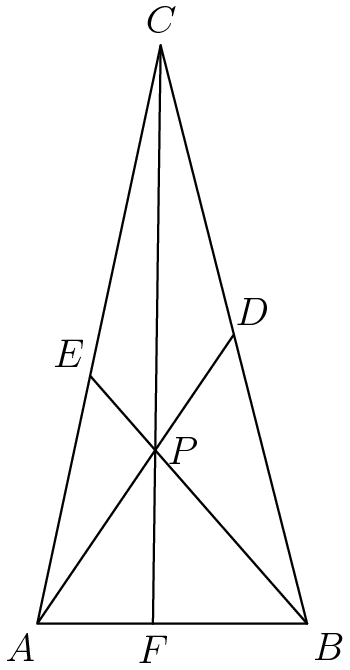
\includegraphics[width = 35.0mm]{img/fig0.png}
\end{center}